\documentclass[10pt]{article}
\usepackage{graphicx, amsthm}
\usepackage{amsmath}
\usepackage[notblind]{optional}
\usepackage[nodayofweek]{datetime}
\usepackage{amsfonts}
\usepackage{amssymb}
\usepackage{xfrac}
\usepackage{caption}
\usepackage{setspace}
\usepackage{multirow}
\usepackage[left=1in, right=.9in, top=.9in, bottom=1in]{geometry}
\usepackage[sort]{natbib}
\usepackage{lscape}
\usepackage[english]{babel}
\usepackage{longtable}
\usepackage{booktabs}
\usepackage{dcolumn}
\usepackage{lscape}
\usepackage{rotating}
\usepackage{setspace}
\usepackage{ifthen}
\usepackage{longtable}
\usepackage{ltxtable}
\usepackage{tabularx}
\usepackage[final]{changes}
\usepackage{tikz}
\usetikzlibrary{snakes}
\usepackage{verbatim}
\newcolumntype{Y}{>{\raggedright \arraybackslash}X}
\newcolumntype{Z}{>{\centering \arraybackslash}X}
\usepackage{titling}
\usepackage{hyperref}
\usepackage[labelfont=bf]{caption}
\usepackage[font=footnotesize]{caption}
\usepackage[font=footnotesize]{subcaption}
\graphicspath{{Images//}}
\usepackage{tcolorbox}
\usepackage{framed}
\usepackage{xcolor}
\usepackage{soul}
\usepackage{mathtools}
\usepackage{float}


\usepackage[utf8]{inputenc}

\title{ML Project}
\author{Tuhin Harit \& Serena Xiao }
\date{May 2021}

\doublespacing
\begin{document}

\maketitle

\section{Introduction}
A recent article in WSJ “Green Euphoria may cost investors, but Planet says Thank you” reported that there is considerable amount of capital $\$80$ billion followed into environmental, social and governance i.e. ESG funds in the third quarter of 2020. These funds only invest in companies that pass the stringent tests on meeting the ESG criteria – a group of standards used by socially conscious investors to screen investments. 



% move this to ppt 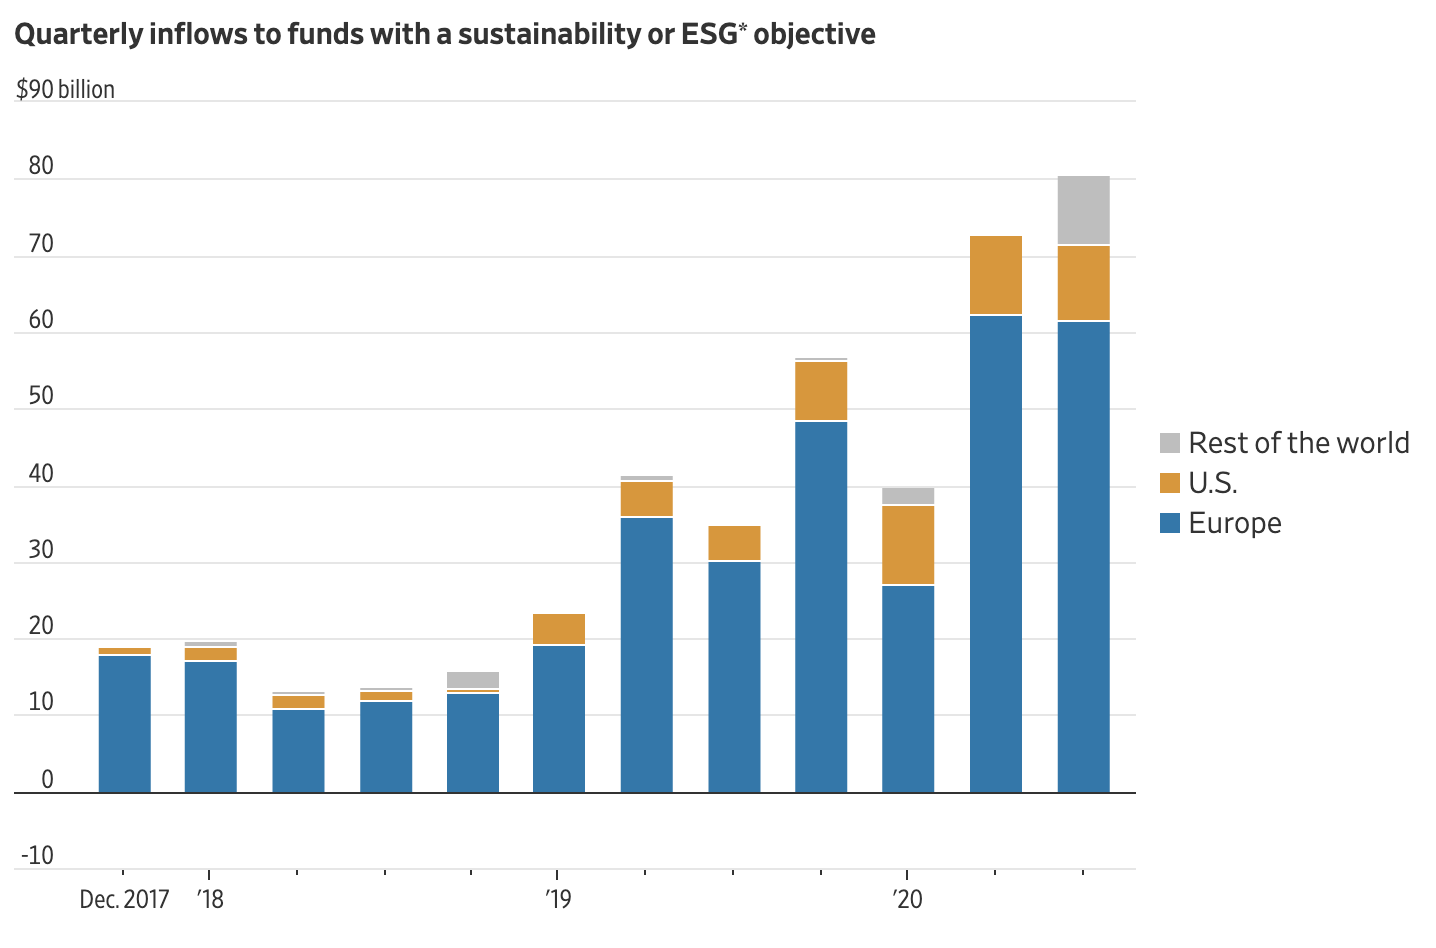
\includegraphics[height=8cm, width=12cm]{fundflow.png}\\
%{\footnotesize source: wall street journal }



Bubble in stock prices of the “green” companies has been a long concern for investors in this space. A fund tracking Nasdaq clean energy index had risen 191\% between end of 2019 to early 2021, which is more than ten times higher than the gain from the broad market index. Quoted from this article: “Private markets generally provide too little incentive for risky innovation because shareholders only capture a small part of an innovation’s benefit; most goes to consumers (think of a life-saving drug)”. For the past decades, there have been increasing number of empirical studies exploring the relationship  between firm performances and green innovation. However, the results are mixed, and it remains ambiguous how or whether the adoption of green innovation would affect a firm’s performance. One obstacle that the researchers are facing in this area is the definition and measure of “green innovation”. 

Our main contribution to the literature is to adapt a relatively newer approach to measure “green innovation”. Following the approach described in Li et al 2020, we adopt their technique to quantify text by using the word embedding model (Mikolov et al, 2013, aka word2vec). Based on the seed words and the texts extracted from the earnings call transcripts, we are able to construct a “green innovation dictionary”. Then based on the frequency count of these words and phrases in the earnings call transcripts, we can generate scores for each firm-quarter. We contrast our measure with Green innovation measure constructed from Loughran and McDonald, 2011 (L\&M) which uses a hand-collected dictionary seeded by "most frequently used words" from an authoritative literature on green innovation.


Our proposed measure using the machine learning approach provides a comprehensive scoring system. On one hand, this score considers the existing green product and process innovation within a firm, which are the two main categories have been studied in the existing papers. On the other hand, it captures the potential of future green development in the firm. We find that our measure of green innovation is significantly able to explain the "actual green innovation" by firms.


\section{Related literature}

Most of the existing research has either used a specific proxy for environmental performance of the firm or considered green innovation in two separate categories: green product v.s. process innovation. For example, Lee et al. 2015 studied the impact of CO2 emissions on firm performance. Driessen et al. 2013 and Albino et al. 2012 examine the green product innovation, and Tseng et al 2013 focuses specifically on the green process innovation. Focusing on one specific area of green innovation is sometimes problematic, as it is difficult to disentangle the effect from green product innovation, green process innovation and overall green policy adopted by the company. When green innovation exists in multiple areas within a firm, there could be spill-over effect. That motivates us to propose one single measure to measure the overall exposure of the firm to “green technology”. 

As mentioned previously, Loughran and McDonald (2011) use a hand-collected dictionary and use it to predict innovation measure. We closely follow the method proposed by Li et al (2020) for measuring innovation and extend it on green innovation and find that it works well in capturing innovation of firms with previous ESG activism (green firms).





\section{Data}
We select the companies with past ESG shareholder proposals. The sample period is 2005-2020. Our earnings call transcripts data are from WRDS database. We have included 14500 transcripts in our sample. The alternate (older) green innovation measure by L\&M that needs hand-created dictionary seeded with most frequently occuring words derived from authoritative texts including research paper(E.g. The Driver of Green Innovation and Green Image: Green Core Competence by Chen et al 2008) and books (Assessment of Carbon Footprint in Different Industrial Sectors by Muthu).

Our algorithm counts the number of mentions of our generated “green innovation” dictionary words in a transcript (Term Frequency - TF). We also generate TF-IDF which evaluates a word's relevance to a document in a collection of documents. (This is done by multiplying two metrics: how many times a word appears in a document, and the inverse document frequency of the word across a set of documents). We also do WF-IDF which uses the log of term frequency in the numerator.


\section{Methodology}

We want to see how well our measure of green innovation (adapted from Li et al(2020)), performs in "actual" green innovation. In absence of a ready-made measure of "actual" green innovation, we use the R\&D expenditure by green firms as the proxy for actual green innovation. We define green firms as those which have ESG activism in the past or future.


We follow the procedure adopted in Li et al. (2020) by applying the the Word2vec model introduced in Mikolov et al (2013) to calculate the word embedding vectors. Word2vec is a technique for natural language processing, which uses a neural network model to learn the word associations. It is an algorithm that takes text corpus as an input and outputs a vector representation for a given word. It utilizes neural network to train itself by reading through the texts in the earnings call transcripts. The training objective is to have the minimum prediction error across all context words in the outer layer. 
\\



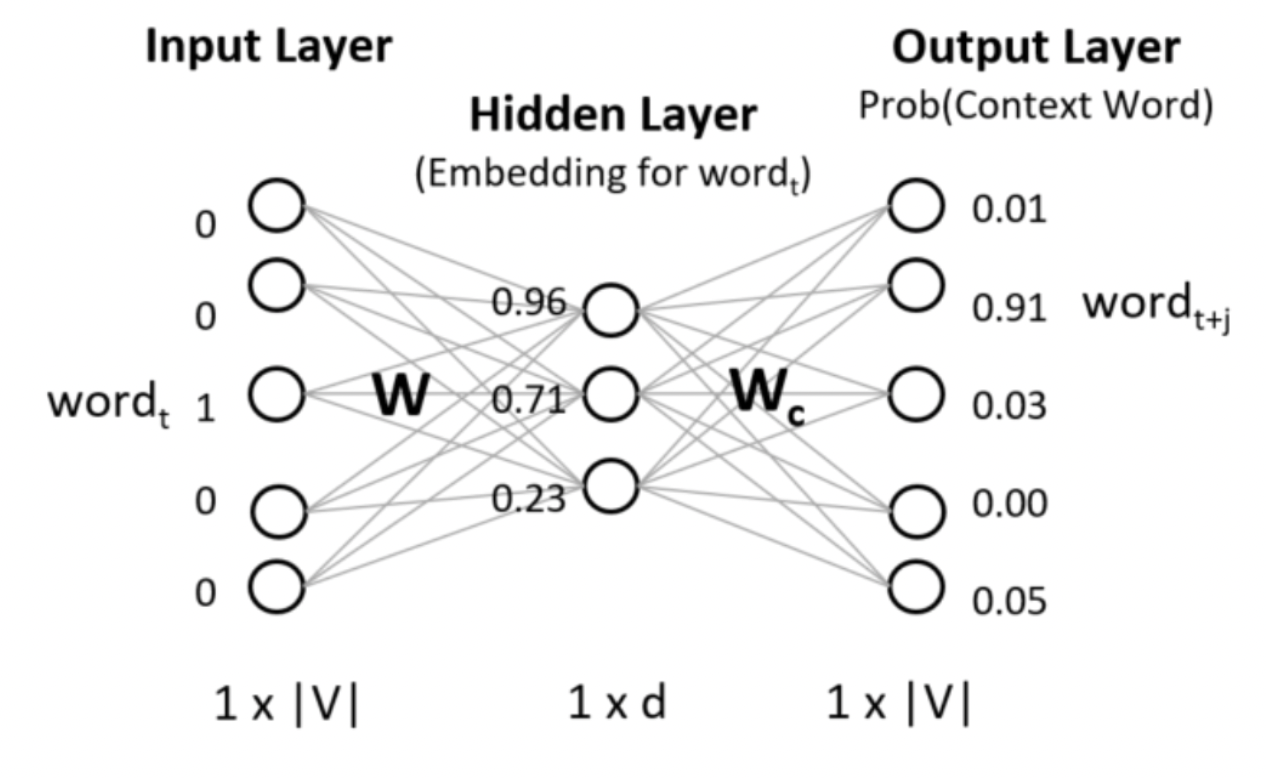
\includegraphics[height=6cm, width=10cm]{word2vec.png}\\
{\footnotesize source: Measuring Corporate Culture Using Machine Learning, Li et al 2018 }

The ultimate goal of the model is to predict neighboring words given an word input. It is equivalent to maximize the average log probability: 

\[\frac{1}{T}\sum^{T}_{t=1}\sum_{-c\leqj\leq c,j\not=0} log(w_{t+j}|w_{t})\]
c is the size of the training context, larger c can result in higher accuracy with larger amount of training time

Context window decides the range in terms of number of words that will be included as context words. We consider a word as “neighbor” if it is within five words from a given word. 
Choosing higher dimension typically increases quality of word embedding, however the marginal gain diminishes. In our project, we choose our dimension to be 100. That means a word embedding coverts to a 100-dimensional vector that represents the meaning of the word. We use cosine similarity to quantify the distance between two words:
\[cosine(A,B) = \frac{A\cdot B}{||A||||B||}=\frac{
\sum^{100}_{i=1}A_{i}B_{i}}{\sqrt{\sum^{100}_{i=1}A_{i}^{2}}\sqrt{\sum^{100}_{i=1}B_{i}^{2}}}\]

where $A_{i}$ and $B_{i}$ are components of vector A and B. 
The vectors are chosen such that the cosine similarity between the vectors measures the level of semantic similarity between the words represented by these vectors. After cosine similarity is calculated between any sets of words, we apply the commonly used method in information retrieval literature - bootstrapping to construct the green innovation dictionary. 


After the dictionary is generated, we apply three different methods of calculating the score for each transcript: raw count, TF-IDF and TF-IDF with log normalization (WF-IDF). The raw scored is the frequency of dictionary words normalized by the total number of words. TF-IDF is a scoring measure that has the advantage to evaluate how important a word is to a document in a collection of documents. This measure is calculated by multiplying word frequency in a document with the inverse document frequency of a word across a set of documents. 

As discussed previously, the alternate L\&M measure requires hand-picked dictionary seeded from most frequently occuring words from representative text on green innovation topic. Once the seed-words are obtained, "hand-picking" is needed to cover the different grammatical forms of the sentiment within the same sentiment (for e.g. if technology is a green innovation seed-word, then technological (adj) and technologically (adverb) should also be "hand-picked" and included in green-innovation dictionary).

\section{Results and discussion}
\underline{Dictionary comparison with althernative method}\\
As mentioned in methodology section, in absence of a direct measure we use r\&d in green firms, which we define as firms that have atleast one occurrence of ESG motions, as a proxy of "actual" green innovation. Additionally, to highlight the superiority of our method over previous method used in finance literature (primarily L\&M) we generate green innovation score using L\&M. 

Table below shows the top 20 words in the dictionary generated by these two methods. Out of these top 20 words, only 7 of them have appeared in both dictionaries. There are only 10 common words that appear in the top 60 words in both dictionaries (16.7\%). We consider the word embedding model is a more advanced technique in our context, as it has the ability to learn the meaning of the words used in the transcripts. It is more of a predictive model, whereas the alternative (LM) method is a count-based model. Dictionary generated by LM method involves many general words that are not closely tied to green innovation, such as ``value'', ``role'', ``case'', etc. In contrast, words dictionary generated by word2vec are more topically related. 
 \\
 \\
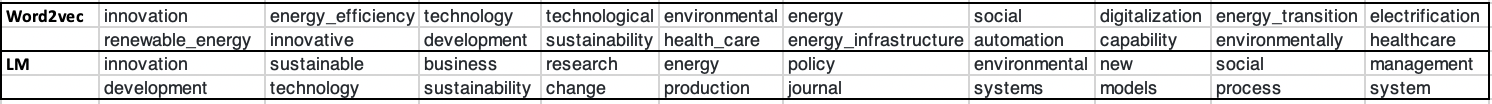
\includegraphics[height=1.5cm, width=18cm]{dict.png}\\
\\
\underline{Validation results}\\
To evaluate whether our measure truly capture the R\&D effort and overall company strategy related to green innovation, we validate our results by using R\&D expenses in the Compustat database. Green innovation spending should be part of the R\&D expenses incurred by any company. We normalize R\&D expense by company's revenue. Table below presents the results of validation tests using both the word2vec and L\&M method. We show that both the contemporaneous and one-quarter lagged green innovation scores based on word2vec method are significantly positively correlated with the R\&D expenses. This positive relation remains significant after control for industry and year fixed effect. In comparison, the green innovation index generated using L\&M method does not show any significant association with the R\&D expenses. These results suggest that the green innovation score generated by this word embedding model works as expected. 
\\


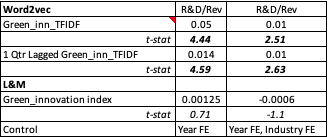
\includegraphics[height=5cm, width=10cm]{validation.png}\\
The results are equally significant for TF and WF-IDF.
 
\section{Conclusion}
To conclude, we are able to extend Li et al (2020) results to create a measure of green innovation which effectively captures the actual green innovation in firms. We find that our measure is more effective in capturing green innovation compared to the traditional L\&M measure. We assign this to superior ability to Word2vec to capture nuanced meanings of words and phrases which the previous methods lacked.

For future work, we would like to test our measure against more direct green innovation proxy (such as green patents). We would like to increase our dataset to include all firms (even those without ESG motions). We would also like to include a more effective benchmark to test the robustness of our results. A natural extension of this research is to use this measure to predict company performance.




\begin{thebibliography}{9}


\bibitem{albino}
Albino, V., Balice, A., & Dangelico, R. M.
\textit{Environmental strategies and
green product development: an overview on sustainability‐ driven companies}. 
Business Strategy and the Environment, 18(2), 83-96, 2012.

\bibitem{driessen}
Driessen, P. H., Hillebrand, B., Kok, R. A., Verhallen, T. M.
\textit{Green new
product development: the pivotal role of product greenness}. 
IEEE Transactions on
Engineering Management, 60(2), 315-326, 2013.

Horváthová, E.
\textit{Does environmental performance affect financial performance? A meta-analysis}.
Ecological Economics 70(1), 52-59, 2010.


\bibitem{wsj} 
 Green Euphoria May Cost Investors, but Planet Says Thank You 
\\\texttt{https://www.wsj.com/articles/green-euphoria-may-cost-investors-but-planet-says\
-thank-you-11609949560}



\bibitem{li} 
Kai Li, Feng Mai, Rui Shen, Xinyan Yan. 
\textit{Measuring Corporate Culture Using Machine Learning}. 
The Review of Financial Studies, 2020.


\bibitem{lee} 
Ki-Hoon Lee, Byung Min, Keun-Hyo Yook. 
\textit{The impacts of carbon (CO2) emissions and environmental research and development (R\&D) investment on firm performance}
International Journal of Production Economics, 167, 2015.


\bibitem{mikolov} 
Mikolov, T., I. Sutskever, K. Chen, G.S. Corrado, and J. Dean. 
\textit{Distributed representations of words
and phrases and their compositionality}. 
Advances in Neural Information Processing Systems, 3111-
3119, 2013.



\end{thebibliography}

\end{document}
